\documentclass[10pt]{beamer}
\usetheme{metropolis}
% all imports
\usepackage[utf8]{inputenc}
\usepackage[T1]{fontenc}
\usepackage{lmodern}
\usepackage{amsmath}
\usepackage{hyperref}
\usepackage{booktabs}
\usepackage{bm}
\usepackage[scale=2]{ccicons}
\usepackage[outputdir=build]{minted}
\usepackage{pgfplots}
\usepackage{array,colortbl,xcolor}
\usepgfplotslibrary{dateplot}
\usepackage{setspace}
\usepackage{etoolbox}
\usepackage{xspace}
\usepackage{tikz}
\usetikzlibrary{shapes,arrows,positioning,fit,backgrounds}
\usepackage{tkz-euclide}

\AtBeginEnvironment{quote}{\singlespacing}

\AtBeginEnvironment{quote}{\singlespacing}

% new commands
\newcommand{\vect}[1]{\bm{#1}}
\newcommand{\myprime}[1]{{#1}^{\prime}}
\newcommand{\grad}[2]{\nabla_{#1} {#2}}
\newcommand{\dotp}[2]{{#1}^{\top}{#2}}
\newcommand{\dotpPright}[2]{{#1}^{\top}\left({#2}\right)}
\newcommand{\outerp}[2]{\left({#1}\right){#2}^{\top}}
\newcommand{\Jacobian}[2]{\frac{\partial #1}{\partial #2}}
\newcommand{\Vocab}{\mathbb{V}}
 \DeclareMathOperator*{\argmin}{arg\,min}
 \DeclareMathOperator{\E}{\mathbb{E}}

% definitions
\definecolor{blue}{RGB}{159, 192, 176}
\definecolor{green}{RGB}{160, 227, 127}
\definecolor{orange}{RGB}{243, 188, 125}
\definecolor{red}{RGB}{253, 123, 84}
\definecolor{nephritis}{RGB}{39, 174, 96}
\definecolor{emerald}{RGB}{46, 204, 113}
\definecolor{turquoise}{RGB}{39, 174, 96}
\definecolor{green-sea}{RGB}{22, 160, 133}
\definecolor{purple}{RGB}{181, 124, 215}
% Tikzstyles for Computation Graphs

% nodes
\tikzstyle{noop} = [circle, draw=none, fill=red, minimum size = 10pt]
\tikzstyle{op} = [circle, draw=red, line width=1.5pt, fill=red!70, text=black, text centered, font=\bf \normalsize, minimum size = 25pt]
\tikzstyle{op2} = [circle, draw=orange, line width=1.5pt, fill=orange!70, text=black, text centered, font=\bf \normalsize, minimum size = 25pt]
\tikzstyle{op3} = [circle, draw=orange, line width=1.5pt, fill=orange!70, text=black, text centered, font=\bf \scriptsize, minimum size = 7pt]
\tikzstyle{placeholder} = [circle, draw=red, line width=1.5pt, fill=red!30, text=black, text centered, font=\bf  \normalsize, minimum size = 25pt]
\tikzstyle{state} = [circle, draw=blue, line width=1.5pt, fill=blue!70, text=black, text centered, font=\bf \normalsize, minimum size = 25pt]
\tikzstyle{gradient} = [circle, draw=nephritis, line width=1.5pt, fill=nephritis!60, text=black, text centered, font=\bf \normalsize, minimum size = 25pt]
\tikzstyle{gradient2} = [circle, draw=green2, line width=1.5pt, fill=green2!60, text=black, text centered, font=\bf \normalsize, minimum size = 25pt]
\tikzstyle{textonly} = [draw=none, fill=none, text centered, font=\bf \normalsize]

% edges
% \tikzstyle{tedge}  = [draw, thick, >=stealth, ->]
\tikzstyle{tedge}  = [draw, thick, >=latex, ->]
\tikzstyle{tedge_dashed}  = [draw, thick, >=latex, ->, dashed]

% namedscope
\tikzstyle{namedscope} = [circle, draw=orange, line width=1.5pt, fill=orange!60, align=center, inner sep=0pt]

% \tikzstyle{container} = [draw=none, rectangle, dotted, inner ysep=1.5em]
% \tikzstyle{novertex} = [draw=none, fill=none, text centered]
% \tikzstyle{predicate} = [ellipse, draw, thick, text centered, rounded corners, minimum size=30pt]
% \tikzstyle{aux} = [rectangle, draw, thick, text centered, rounded corners, minimum size=30pt]
% \tikzstyle{ledge}  = [draw, dashed, thick, >=stealth, ->]
% \tikzstyle{pedge}  = [draw, thick, >=stealth, ->]


\title{Adding semantic robustness\\ to dialog agents}
\date{\today}

\vspace{1.1 cm}


\author{
  Felipe Salvatore\\
  \url{https://felipessalvatore.github.io/}
  \vspace{1.1 cm}}

\institute{\textbf{IME-USP}: Instituto de Matemática e Estatística - Universidade de São Paulo}


\begin{document}
\nocite{DeepLearningbook}


\maketitle


\begin{frame}{Sistemas de diálogo}
 criar um programa capaz de dialogar com ser humano
\begin{center}
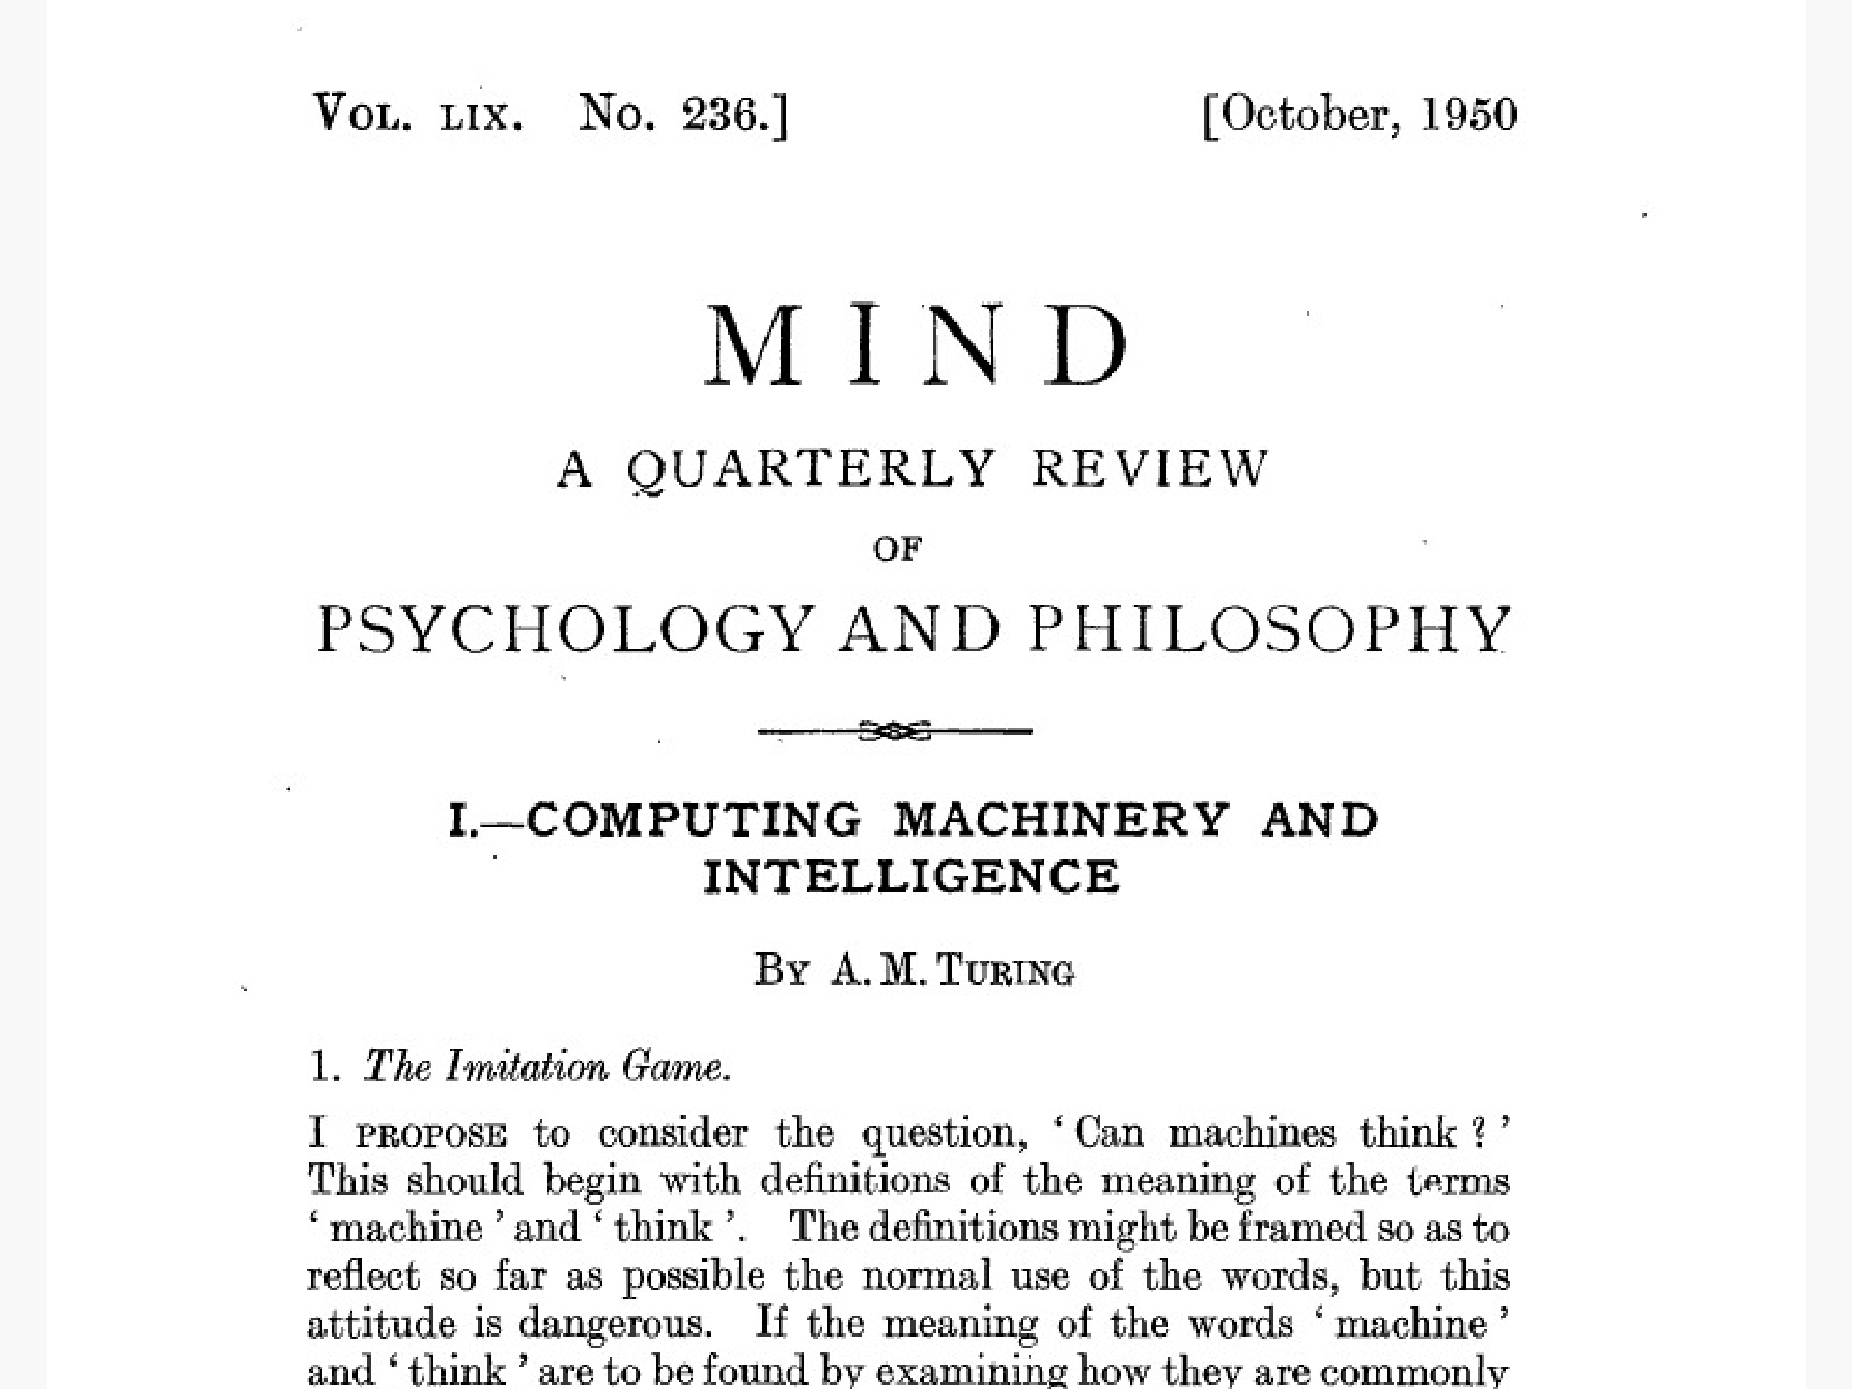
\includegraphics[scale=0.16]{images/turing.jpg}
\end{center}
\end{frame}


\begin{frame}{Sistemas de diálogo}
goal -driven vs non-goal driven
\end{frame}


\begin{frame}{Modelos de linguagem baseados em redes neurais}
Nos chamamos de \alert{modelo de linguagem} uma distribuição de probabildiade sobre uma sequencia de tokens em uma lingua natural.

\[
P(x_1,x_2,x_3,x_4) = p
\]

Em vez de usar uma abordagem que seja específica para o domínio da linguagem natural, podemos usar um modelo para predição de dados sequencias:  \textbf{uma rede recorrente (RNN)}. \\

Nossa tarefa de aprendizado é estimar a distribuição de probabilidade

\[
P(x_{n} = \text{palavra}_{j^{*}} | x_{1}, \dots ,x_{n-1})
\]

para qualquer $(n-1)$ sequencia de palavras $x_{1}, \dots ,x_{n-1}$.

\end{frame}

\begin{frame}{O modelo de linguagem com RNN}
% RNN STATE CELL ====================================
\newcommand{\rnnSimpleU}[4]{

% operations
\node[state, minimum size=40pt,#4] (h#3) {$\vect{h}^{#1}$};
\node[op, minimum size=40pt, above=30pt of h#3] (yhat#3){$\hat{\vect{y}}^{#1}$};
\node[op, minimum size=40pt,below=30pt of h#3] (e#3) {$\vect{e}^{#1}$};
\node[textonly, below=0.1pt of e#3] {{\Large#2}};

% edges
\path[tedge] (e#3) edge node[below right= -4pt] {$\vect{U}$} (h#3);
\path[tedge] (h#3) edge node[below right = -4pt] {$\vect{V}$} (yhat#3);
}

\begin{figure}[ht!]
\hspace*{-1.0cm}
\scalebox{0.8}{
\begin{tikzpicture}[auto]

% timestep 1
\rnnSimpleU{(1)}{Yes}{t1}{}

% % timestep 0
\node[state, minimum size=40pt,left=50pt of ht1] (ht0) {$\vect{h}^{(0)}$};

% % timestep 2
\rnnSimpleU{(2)}{here}{t2}{right=50pt of ht1};


% % timestep 2
\rnnSimpleU{(3)}{we}{t3}{right=50pt of ht2};


% % state transfers
\path[tedge] (ht0) edge node[above right = 2pt] {$\vect{W}$} (ht1);
\path[tedge] (ht1) edge node[above right = 2pt] {$\vect{W}$} (ht2);
\path[tedge] (ht2) edge node[above right = 2pt] {$\vect{W}$} (ht3);

% % text
\node[textonly, above=40pt of yhatt2] (result) {{\Large $P(x^{(4)}| \text{Yes, here, we})$}};

% Arrow to result
\draw[->, line width=1mm] [bend right, out=-50, distance=25pt](yhatt3.north) to  (result.east);


\end{tikzpicture}
}%\scalebox
\end{figure}


\end{frame}



\begin{frame}{GRU: Gated Recurrent Units}
\begin{center}
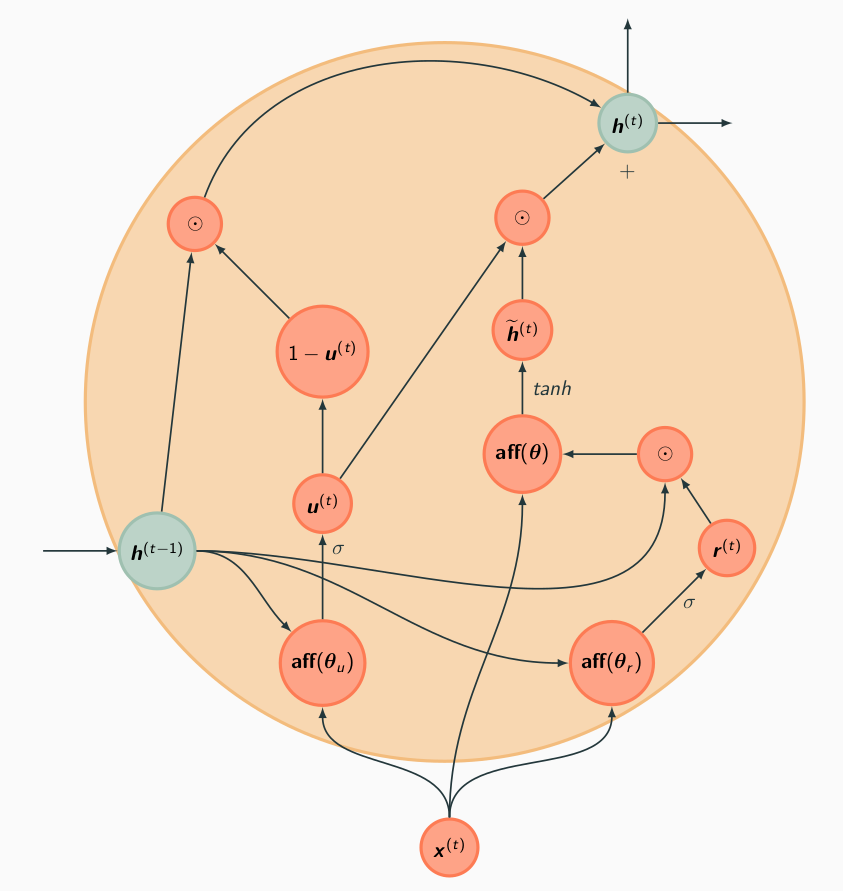
\includegraphics[scale=0.25]{images/gru.png}
\end{center}
\end{frame}


\begin{frame}{LSTM: Long Short Term Memory}
\begin{center}
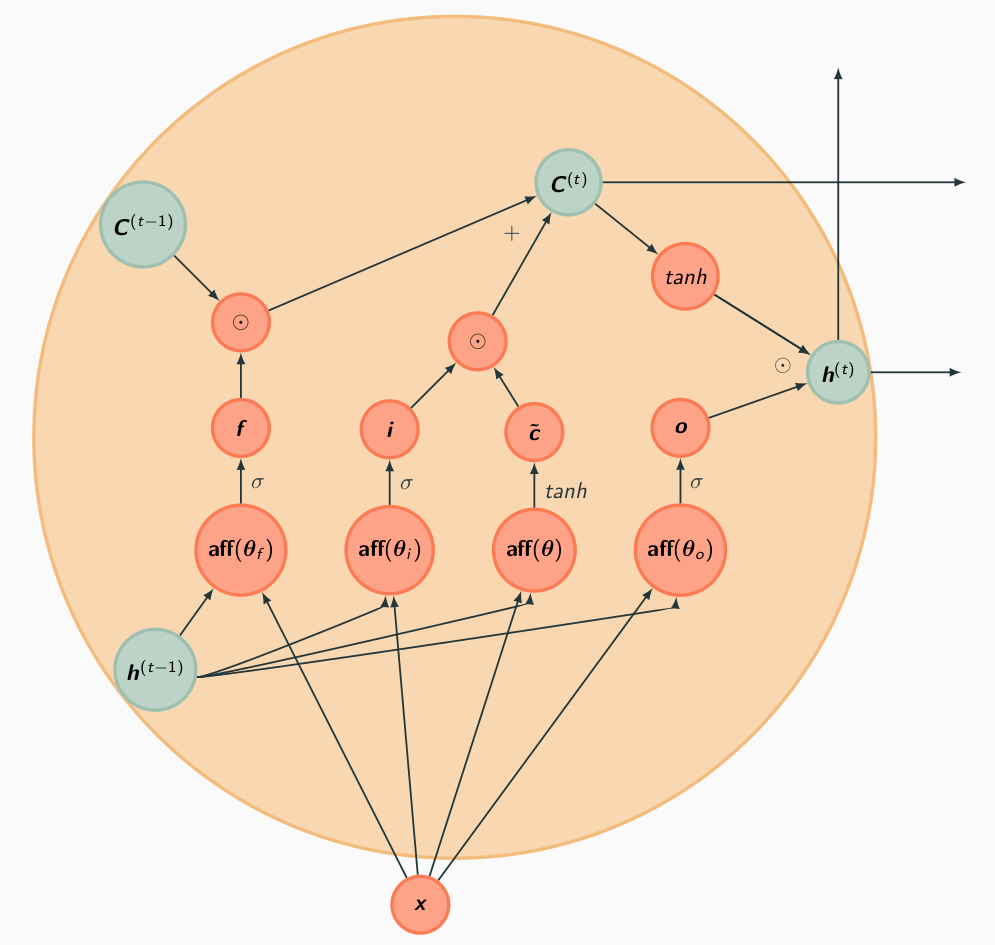
\includegraphics[scale=0.23]{images/lstm.png}
\end{center}
\end{frame}


\begin{frame}{Exemplo: TrumpBot\\\url{https://github.com/felipessalvatore/MyTwitterBot}}
\begin{center}
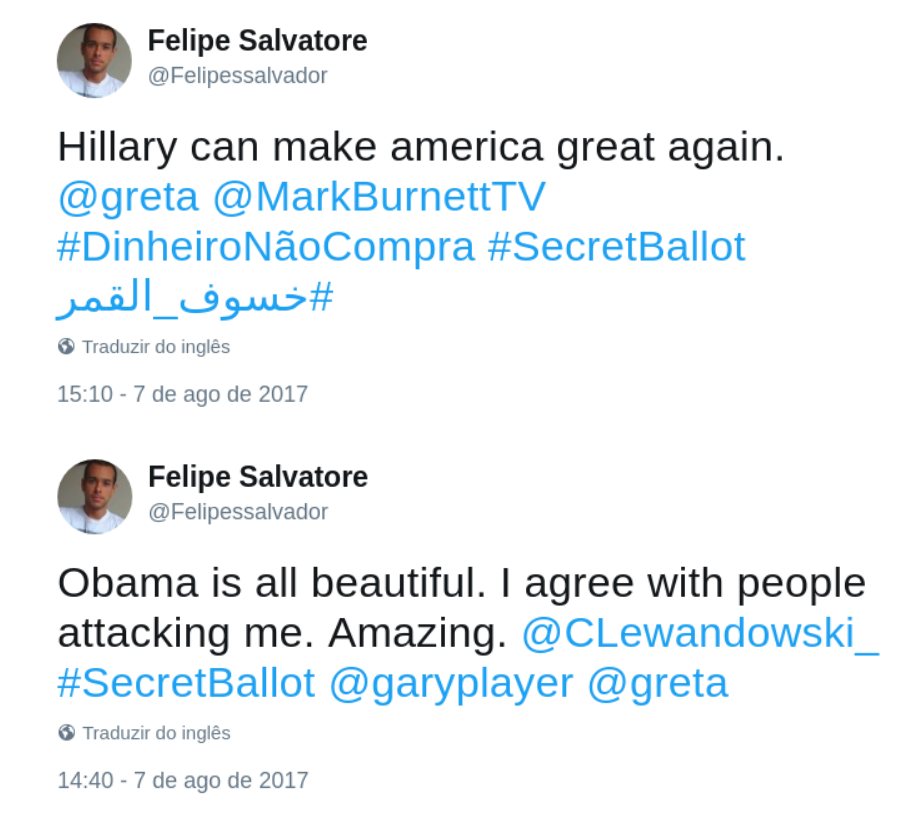
\includegraphics[scale=0.24]{images/TrumpBot.png}
\end{center}
\end{frame}


\begin{frame}{Exemplo: Funk Generator\\ \url{https://github.com/lucasmoura/funk_generator}}
\begin{quote}
\centering
É o dj que tá tocando e não sabe de nada\\ 
Eu já tô no clima e já tô no meu nome \\
Cordão de ouro no pescoço eu tô na moda \\
Com a camisa da \\
Louis \\
Vuitton \\
Pulo da morena que elas gosta\\ 
E se eu te pego no baile \\
De captiva de citroen ou de hayabusa\\ 
Tu viu a 1100 cilindradas \\
Se eu tô no litoral de cordão de ouro\\ 
De cordão de ouro no pescoço\\
\end{quote}
\end{frame}


\begin{frame}{Modelos de linguagem baseados em redes neurais}

\end{frame}


\begin{frame}{Modelos de linguagem baseados em redes neurais}

\end{frame}


\begin{frame}[allowframebreaks]{Referências}

  \bibliography{my_references}
  \bibliographystyle{abbrv}

\end{frame}

\end{document}




\end{document}